\chapter{Resultados}

O presente estudo reuniu uma série de aspectos que caracterizam ambos os estilos arquiteturais com
base no que é apresentado nos referenciais teóricos adotados. Dentro dessa base construída de
informação, notou-se níveis diferentes dentre essas características, as quais foram classificadas em
aspectos, impactos, causa e constância na \autoref{sinteses} de acordo com as perspectivas e fatores
adversos identificados para os mesmos.

Nessa abordagem, notou-se nas causas elencadas as características mais básicas de cada estilo
arquitetural. Tais características são para a arquitetura monolítica a simplicidade arquitetural e a
essência de ser um modelo altamente acoplado. É importante compreender que a natureza tecnicamente
estruturada do modelo e a prática de reutilização de código comumente aplicada a esta arquitetura
contribuem para a baixa coesão e o alto acoplamento geralmente encontrado neste estilo.

Do outro lado, os microsserviços têm como características básicas a alta complexidade e o baixo
acoplamento oriundos da sua natureza distribuída e dos conceitos de \gls{DDD}. Para completar, neste
modelo é preferível a duplicação de código entre os serviços, o que contribui para manter a alta
coesão e o baixo acoplamento.

\begin{figure}[h]
  \centering
  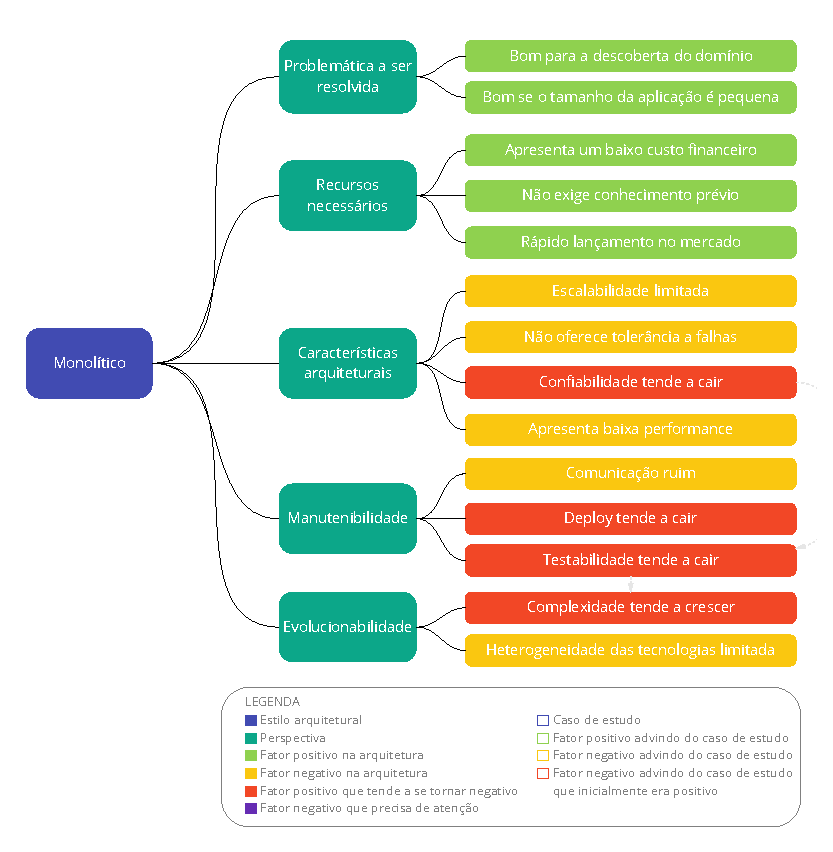
\includegraphics[keepaspectratio=true,scale=1]{figuras/sintese-monolitico.eps}
  \caption{Mapa mental do processo de síntese realizado sobre a arquitetura
  monolítica\label{fig:SinteseMono-resultados}}
\end{figure}

\begin{figure}[h]
  \centering
  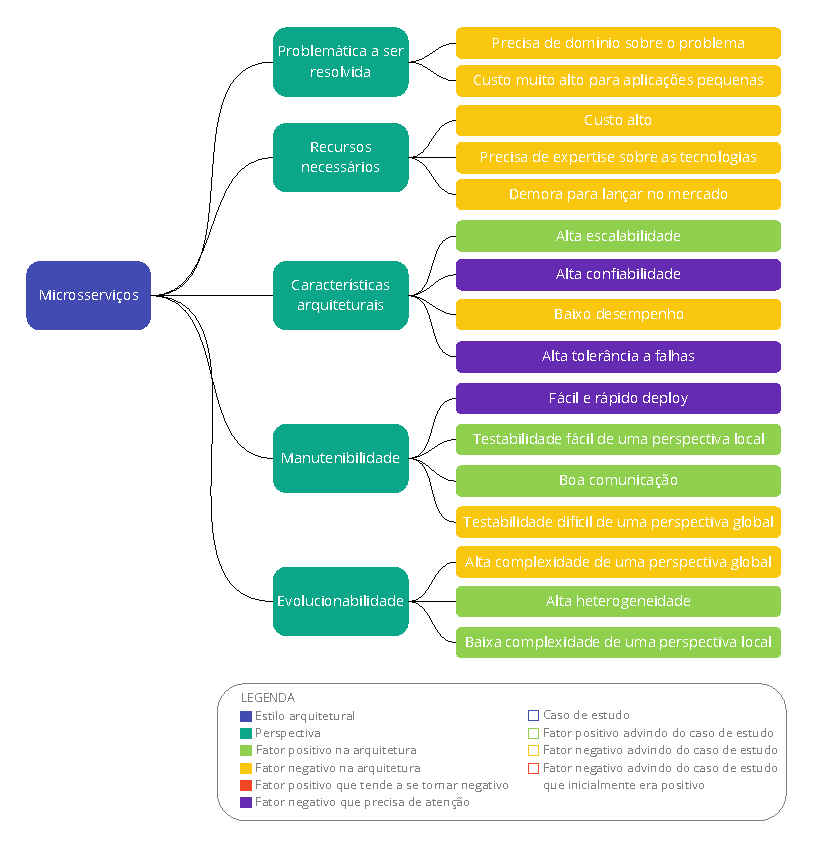
\includegraphics[keepaspectratio=true,scale=1]{figuras/sintese-microsservicos.eps}
  \caption{Mapa mental do processo de síntese realizado sobre a arquitetura de microsserviços\label{fig:SinteseMicro-resultados}}
\end{figure}

A \autoref{fig:SinteseMono-resultados} e a \autoref{fig:SinteseMicro-resultados} apresentam os
diagramas elaborados na \autoref{sinteses}. Ao comparar os dois diagramas, vemos que a arquitetura
monolítica é favorecida em um contexto inicial da aplicação, quando olhamos as perspectivas de
problemática a ser resolvida e recursos necessários, essa arquitetura favorece contextos onde não se
têm domínio sobre o problema, nem grandes recursos financeiros e humanos.

Já a arquitetura de microsserviços, \autoref{fig:SinteseMicro-resultados}, quando analisada diante
desses aspectos, é uma arquitetura que exige mais tempo, planejamento e recursos ao se iniciar um
projeto, visto que é preciso domínio sobre o problema, mão de obra especializada e
automatizar uma série de processos para que a arquitetura seja realmente viável.

Todavia, ao olhar para as perspectivas de características arquiteturais, manutenibilidade e
evolucionabilidade, a arquitetura de microsserviços se destaca em relação a arquitetura monolítica,
apresentando boa escalabilidade, boa comunicação entre os times, etc. Vale destacar que o modelo
arquitetural de microsserviços apresenta uma dualidade que não existe na arquitetura monolítica,
que é a percepção local e global dessa arquitetura. Assim, nota-se aspectos como a testabilidade e a
complexidade que olhando localmente para cada serviço são fatores positivos de lhe dar, porém ao
olhar os mesmos fatores de uma perspectiva global de todos os serviços estes se tornam aspectos
negativos da arquitetura.

Por último, temos os fatores que necessitam de atenção em cada uma das arquiteturas (destacados com as
cores vermelha e roxo nos diagramas). A primeira diferença que se nota ao olhar estes fatores é que
a arquitetura monolítica só possui fatores positivos que tendem a se tornar negativos (vermelhos),
enquanto que a arquitetura de microsserviços só possui fatores positivos que precisam de atenção
(roxo). Esta distinção é essencial para entender o crescimento de cada uma das arquiteturas. Quando
olhamos para os monolíticos, fatores como confiabilidade, testabilidade, são inicialmente bons e
providos pelo modelo arquitetural, contudo eles tendem a decair e não há nada nesse estilo arquitetural
que contribua para minimizar tal aspecto, dependendo unicamente dos desenvolvedores de controlar a
crescente complexidade do sistema.

Na arquitetura de microsserviços, vemos os fatores de confiabilidade, tolerância a falhas e \textit{deploy}
como os fatores que precisam de atenção. Neste caso, entende-se que existem meios de contornar essas
questões que não dependem unicamente do dia-a-dia dos desenvolvedores. Por exemplo, a confiabilidade
e a tolerância a falhas podem ser garantidas mediante estratégias para lhe dar com a sobrecarga da
rede, já a facilidade do \textit{deploy} é garantida se você automatizar os processos.

Ao olharmos para os casos práticos, percebe-se experiências que atestam as características elencadas
pelos referenciais teóricos, como a complexidade dos monolíticos quando a base de código se torna
volumosa, relatado pela Otto e pelo KN Login, ou a alta tolerância a falha dos microsserviços
apresentada nos casos da Otto e da Segment. Percebe-se também, outros aspectos comuns da arquitetura
abordados pelos casos práticos como a curva de aprendizado sobre o sistema que tende a ser maior na
arquitetura monolítica, contribuindo para a dificuldade de contratar novos desenvolvedores, ou a
facilidade de receber \textit{feedbacks} e testar novas funcionalidades na arquitetura de
microsserviços após o período inicial de planejar e automatizar todos os processos.

Por fim, voltamos as Leis da Arquitetura de Software abordadas na \autoref{leis}, as quais dizem que
tudo na arquitetura de software é um conflito de escolha e que "por que" é mais importante do que
"como". A escolha de adotar um estilo arquitetural monolítico traz uma série de benefícios no começo
da aplicação, principalmente o tempo de lançamento no mercado que é mais curto e a facilidade de
alterar as funcionalidades nesse início no qual se está descobrindo o domínio da aplicação com os
usuários, contudo, a medida que a base de código cresce essas características vão se perdendo.
Mediante tal situação entra uma análise sobre os objetivos de negócio da empresa e os recursos
disponíveis, se o planejado é manter uma aplicação pequena e simples ou se a empresa não possui muitos
recursos a arquitetura monolítica é a abordagem recomenda, mas se o almejado é ter uma aplicação maior
em um contexto mais complexo ou se a aplicação monolítica está crescendo além do planejado, o mais
recomendado é migrar para outro modelo arquitetural. Nas palavras de Martin Fowler:

\begin{quotation}{MartinFowler:MonolithFirst}{transleted=true}
    Não tenha medo de construir um monolítico que você irá descartar, especialmente se o monolítico
    puder levar você ao mercado rapidamente.\footnote{Texto original: \textit{ Don't be afraid of
    building a monolith that you will discard, particularly if a monolith can get you to market quickly.}}
\end{quotation}

A arquitetura de microsserviços provê um sistema mais sutentável ao longos dos anos
\cite{Guido2016:WhyMicroservices}, porém ela apresenta um alto custo de construção e
manutenção além de exigir que se tenha domínio sobre o contexto e sobre as tecnologias. Desta forma
voltamos ao ponto, defendido na justificativa do presente trabalho, \autoref{justificativa}, de que é preciso analisar o
contexto e os objetivos de negócio da empresa de forma que o modelo arquitetural seja capaz de
auxliar essas empresas a alcançarem seus objetivos.
